\documentclass[aspectratio=169,usenames,dvipsnames]{beamer}
\beamertemplatenavigationsymbolsempty
% \documentclass{beamer}

% UNCOMMENT FOR HANDOUTS
% \usepackage{pgfpages}
% \pgfpagesuselayout{2 on 1}[landscape,letterpaper,border shrink=5mm]
% \setbeameroption{show notes}

\mode<presentation>
\usetheme{Boadilla}
\usecolortheme{spruce}
\usepackage{../LizStyle,ulem}
\usepackage{color}
\usepackage[color,matrix,arrow]{xy}
% \input xy
% \xyoption{all}
\usepackage{tikz}
\usepackage{tikz-cd}
\tikzset{commutative diagrams/diagrams={ampersand replacement=\&}}

\AtBeginSection{\frame{\sectionpage}}


% ==========Command for putting comments and removing them=======
% Visible:
\newcommand{\InstructorNotes}[1]{\textit{\color{orange}#1}}
\newcommand{\InstructorList}[1]{
\begin{itemize}
	\color{orange}
	#1
\end{itemize}
}
% Removed:
\renewcommand{\InstructorNotes}[1]{}
\renewcommand{\InstructorList}[1]{}


\newcommand{\bvfill}{\vskip0pt plus 1filll}

\usepackage{multimedia}
\usepackage{graphbox}

% \usepackage{algpseudocode}


\graphicspath{ {Figures/} {../Figures/}{../../Figures/} }



\begin{document}
%\pdfoptionpdfminorversion 5
%\logo{\includegraphics[height=1.5cm]{dukeshield.pdf}}
\title[]{Ch 5.2: The Bootstrap}
\subtitle{Lecture 16 - CMSE 381}
\date{Wed, Oct 9, 2024}



\institute[MSU-CMSE]{Michigan State University\\
			::\\
          Dept of Computational Mathematics, Science \& Engineering}
\author[Dr.~Munch]{Prof.~Elizabeth Munch}

\begin{frame}
 \titlepage


\end{frame}
%--------------------------
\begin{frame}[c]{Announcements}

\begin{columns}
\column{.45\textwidth}
\centering

	Last time:
	\begin{itemize}
		\item $k$-fold CV for Classification 
	\end{itemize}
\textbf{Announcements:}
	\begin{itemize}
		\item Homework \#4 Due Tonight!
	\end{itemize}
\column{.45\textwidth}
\centering

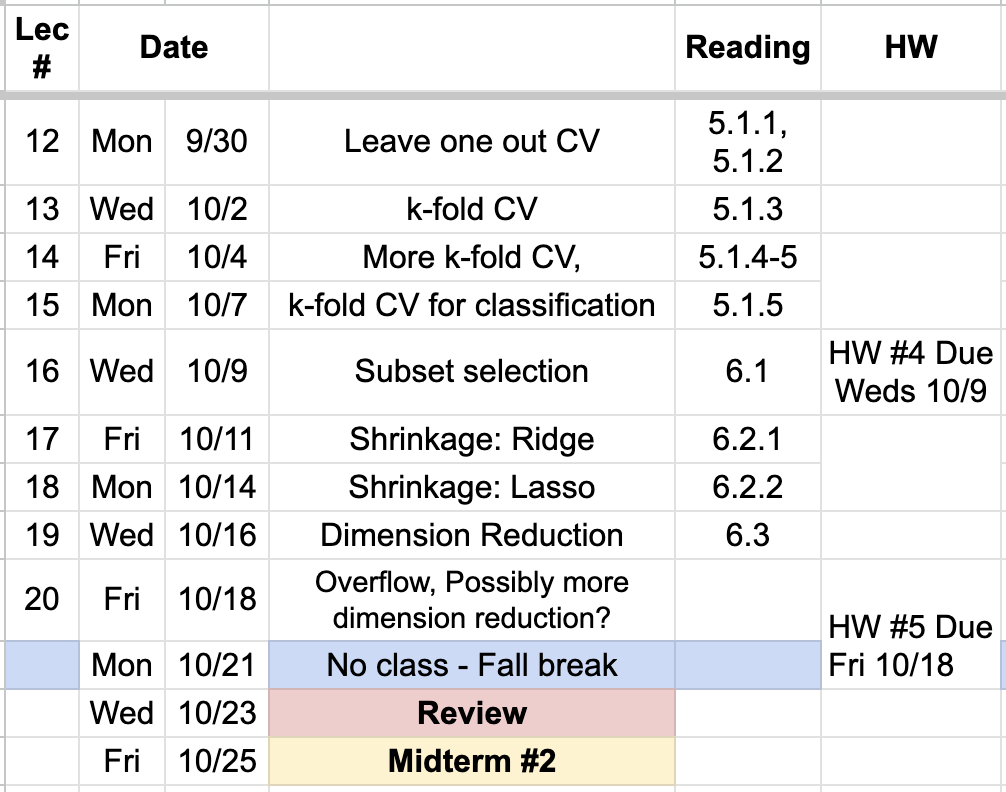
\includegraphics[width = \textwidth]{Day01-Schedule-Test2.png}

\end{columns}

\end{frame}
%--- Next Frame ---%
\begin{frame}[c]{Covered in this lecture }

\begin{columns}
\column{.4\textwidth}
\centering
\begin{itemize}
	\item Bootstrap
\end{itemize}


\column{.4\textwidth}
\centering
\end{columns}

\end{frame}
%--- Next Frame ---%



%=====
\section{The Bootstrap}
%=====

\begin{frame}[t]{The Idea}

\begin{columns}
\column{.45\textwidth}
\centering

\textbf{The goal:} quantify the uncertainty associated with a given estimator or statistical learning method.

\InstructorNotes{The method: Bootstrap}
\column{.45\textwidth}
\centering
\InstructorList{
\item Can be used to estimate std error of linear regression coefficients, but that's boring since we have other tools
\item the power of the bootstrap lies in the fact that it can be easily applied to a wide range of statistical learning methods,
\item  including some for which a measure of variability is otherwise difficult to obtain and is not automatically output by
statistical software.
}
\end{columns}

\end{frame}
%--- Next Frame ---%
\begin{frame}[c]{The bootstrap idiom}

\begin{quote}
	\centering
	``Pull yourself up by your bootstraps."
\end{quote}
\begin{columns}
\column{.4\textwidth}
\centering
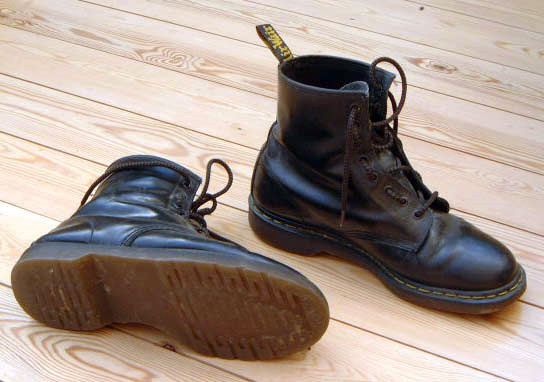
\includegraphics[width = \textwidth]{Dr_Martens,_black,_old.jpg}
\column{.45\textwidth}
\centering
\begin{itemize}
\item Originally used as a saying meaning an impossible task, used sarcastically
\item Now often used to imply that socioeconomic advancement is something everyone should be able to do
\item Also source of the term "booting" a computer
\end{itemize}
\end{columns}

\end{frame}
%--- Next Frame ---%

\begin{frame}[c]{Today's class: Bootstrap on a simple modeling problem}

\begin{columns}
\column{.45\textwidth}
\centering
\begin{itemize}
	\item
We wish to invest a fixed sum of money in two financial assets that yield returns of $X$ and $Y$, respectively, where $X$ and $Y$ are random quantities.
\item We will invest a fraction $\alpha$ of our money in $X$, and will
invest the remaining $1-\alpha$ in $Y$.
\item  Since there is variability associated with the returns on these two assets, we wish to choose $\alpha$ to minimize the total risk, or variance, of our investment.
\end{itemize}

\column{.45\textwidth}
\centering
\InstructorNotes{
Really: want to minimize $\Var(\alpha X + (1-\alpha)Y)$
}
\end{columns}

\end{frame}
%--- Next Frame ---%
\begin{frame}[c]{One can show.....}

\begin{columns}
\column{.45\textwidth}
\centering
...that
$\Var(\alpha X + (1-\alpha)Y)$

is minimzed by

\begin{equation*}
	\alpha = \frac{\sigma_Y^2 - \sigma_{XY}}{\sigma_X^2 + \sigma_Y^2 - 2\sigma_{XY}}
\end{equation*}
where
\begin{itemize}
	\item $\sigma_X^2 = \Var(X)$
	\item $\sigma_Y^2= \Var(Y)$
	\item $\sigma_{XY} = \mathrm{Cov}(X,Y)$
\end{itemize}
\column{.45\textwidth}
\centering
Get an estimate:
\begin{equation*}
	\hat\alpha = \frac{\hat\sigma_Y^2 - \hat\sigma_{XY}}{\hat\sigma_X^2 + \hat\sigma_Y^2 - 2\hat\sigma_{XY}}
\end{equation*}
\end{columns}

\end{frame}
%--- Next Frame ---%

\begin{frame}[c]{Simulated data }

	\begin{columns}
	\column{.45\textwidth}
	\centering

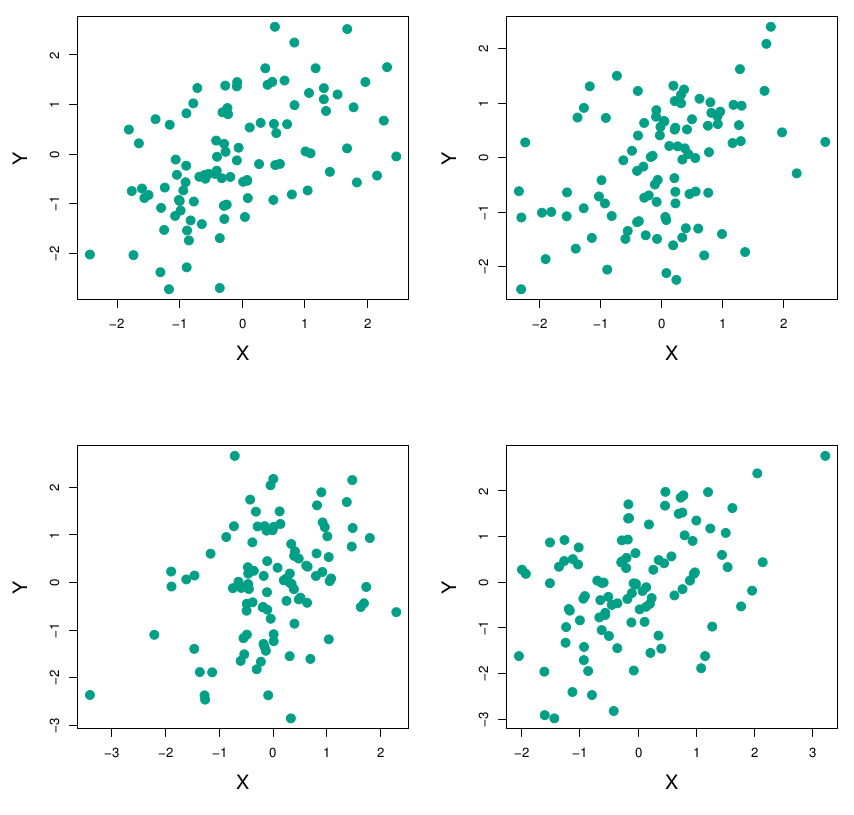
\includegraphics[width = \textwidth]{Fig5-9}
	\column{.45\textwidth}
	\centering
	\begin{itemize}
		\item Simulate data using
		\begin{itemize}
			\item 	$\sigma_X^2 = 1$
			\item $\sigma_Y^2 = 1.25$
			\item $\sigma_{XY} = 0.5$
			\item Implies $\alpha = 0.6$
		\end{itemize}
		\item In each panel: Simulate 100 pairs of returns for investments
		\item Predict $\sigma_X^2$, $\sigma_Y^2$, and $\sigma_{XY}$
		\item
	$\hat \alpha$ prediction by panel:

	$
	\begin{matrix}
		0.576 & 0.543 \\
		0.657 & 0.651
	\end{matrix}
	$
	\end{itemize}

	\end{columns}


\end{frame}
%--- Next Frame ---%
\begin{frame}[c]{Resimulate: Rinse and repeat}

\begin{columns}
\column{.35\textwidth}
\centering
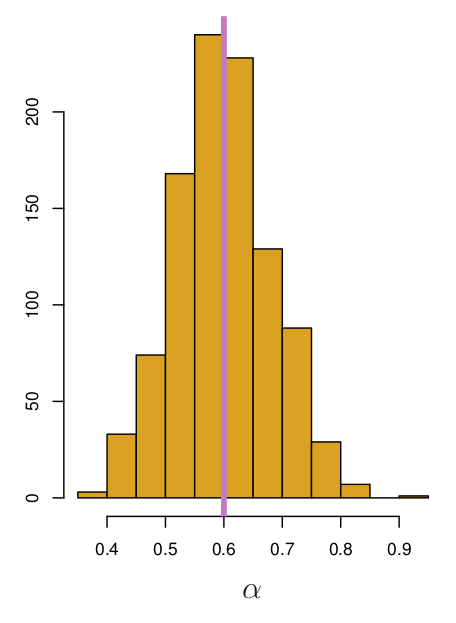
\includegraphics[width = \textwidth]{Fig5-10a}
\column{.45\textwidth}
\centering
\begin{itemize}
	\item Simulate 100 data points 1,000 times
	\item Left: Histogram of predictions for $\alpha$
	\item Pink line: True value for $\alpha$
	\item Mean over simulated values: $0.5996 = \bar \alpha = \frac{1}{1000}\sum \hat \alpha_r$
	\item St dev: $0.083 = \sqrt{\frac{1}{1000-1} \sum (\hat \alpha_r - \bar \alpha)}$
\end{itemize}
\end{columns}

\end{frame}
%--- Next Frame ---%
{
\setbeamercolor{background canvas}{bg=Apricot!25}
\begin{frame}[t]{Coding part 1: Apprximate $\hat \alpha$ with simulated data}
\begin{columns}
\column{.45\textwidth}
\centering
\column{.45\textwidth}
\centering
\end{columns}
\end{frame}
}
%--- Next Frame ---%

\begin{frame}[c]{So what's the problem?}

\begin{columns}
\column{.45\textwidth}
\centering
\InstructorNotes{I can't simulate my data!}
\column{.45\textwidth}
\centering
\InstructorNotes{So the bootstrap plan..... create simulations from the original data set}
\end{columns}

\end{frame}
%--- Next Frame ---%
\begin{frame}[c]{The solution: Sample the data with replacement}


\begin{columns}
\column{.45\textwidth}
\centering

	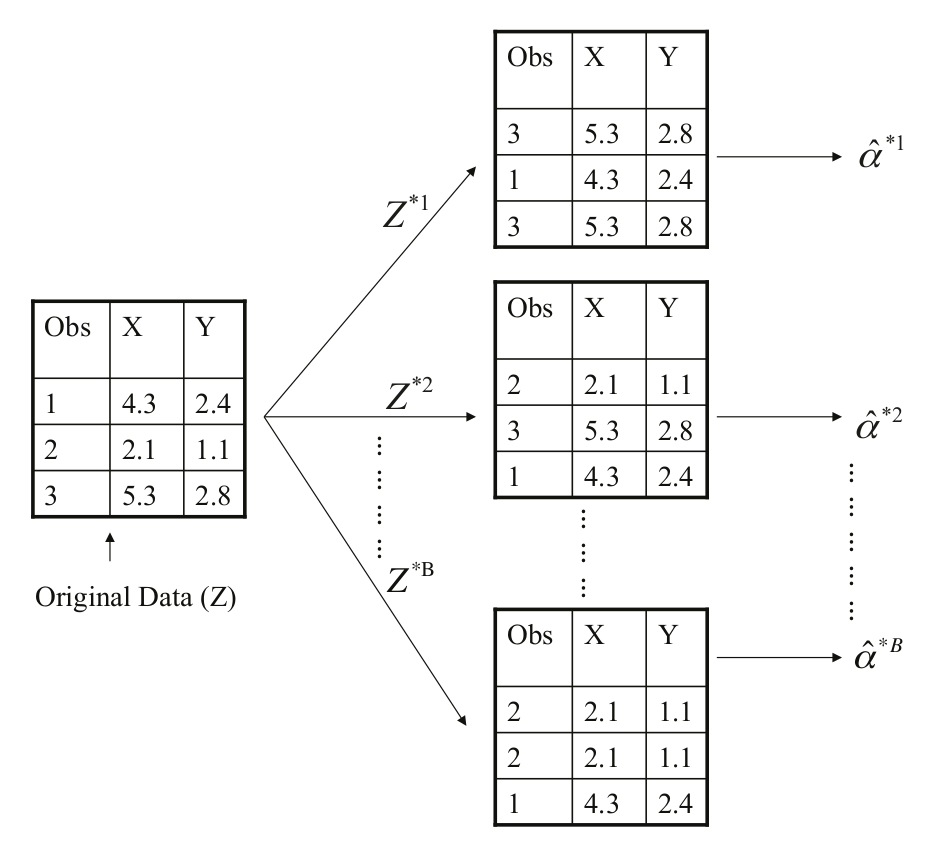
\includegraphics[width = \textwidth]{Fig5-11}
\column{.45\textwidth}
\centering
\InstructorList{
\item Note that data points can show up repeatedly
\item Note that the size of the sample is always $n$, but with repeats
\item Different from the validation set approach since there we had no repeats; also cared more about error than about the models
}
\end{columns}

\end{frame}

%--- Next Frame ---%
\begin{frame}[c]{Computation of error }

\begin{columns}
\column{.35\textwidth}
\centering
\begin{itemize}
	\item Repeate procedure $B$ times:
	\item Get $B$ bootstrap data sets, $Z^{*1},Z^{*2},\ldots,Z^{*B}$
	\item Get $B$ bootstrap estimates
	$\hat\alpha^{*1},\hat\alpha^{*2},\ldots,\hat\alpha^{*B}$
\end{itemize}
\column{.55\textwidth}
\centering
Get standard error estimate:
\begin{equation*}
	SE_B(\hat \alpha) = \sqrt{ \frac{1}{B-1}
	\sum_{r=1}^B \left(
	\hat \alpha^{*r} - \frac{1}{B}\sum_{r'=1}^B \hat \alpha^{*r'}
	\right)^2
	}
\end{equation*}
\InstructorList{
  \item Point out this is the estimate of standard deviation of the alpha hats
  \item If you use `np.std' you need to be careful because it doesn't do divde by N-1 without some extra flag
}

\end{columns}

\end{frame}
%--- Next Frame ---%
{
\setbeamercolor{background canvas}{bg=Apricot!25}
\begin{frame}[t]{Coding part 2: Resampling data}
\begin{columns}
\column{.45\textwidth}
\centering
\column{.45\textwidth}
\centering
\end{columns}
\end{frame}
}
%--- Next Frame ---%
\begin{frame}[c]{Back to the example}

\begin{columns}
\column{.85\textwidth}
\centering
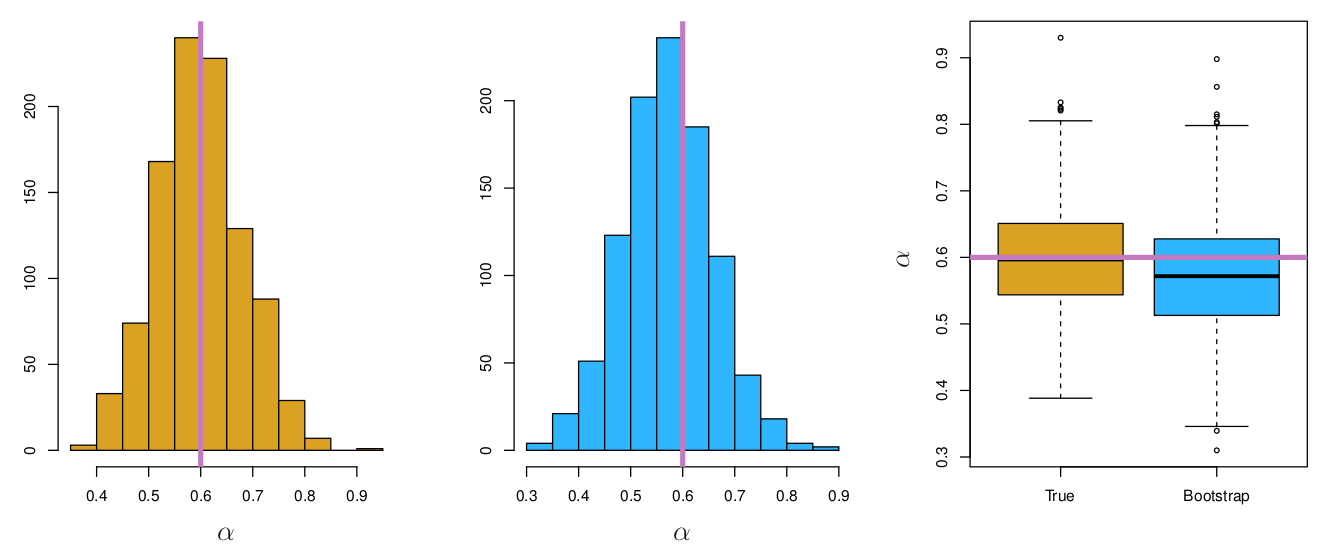
\includegraphics[width = \textwidth]{Fig5-10}
% \column{.45\textwidth}
% \centering

\end{columns}


\begin{columns}
\column{.3\textwidth}
\centering
Resample version \\
Predicted $SE(\hat \alpha) = 0.083$
\column{.3\textwidth}
\centering
Bootstrap version \\
Predicted $SE(\hat \alpha) = 0.087$
\column{.3\textwidth}
\centering
\InstructorNotes{Boxplots have similar spreads, meaning can both be used to estimate the variability of $\hat \alpha$}
\end{columns}


\end{frame}
%--- Next Frame ---%

\begin{frame}[c]{A general picture for the bootstrap}

\begin{columns}
\column{.75\textwidth}
\centering
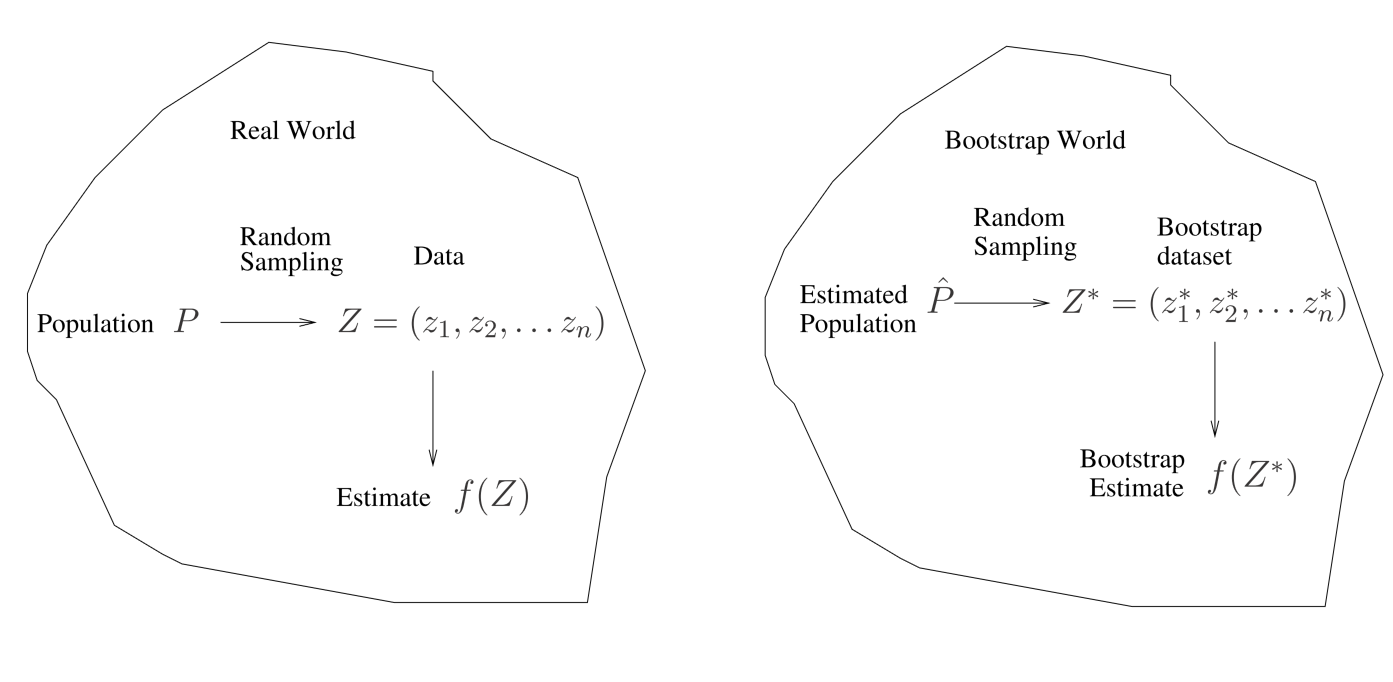
\includegraphics[width = \textwidth]{BootstrapWorld.png}
% \column{.45\textwidth}
% \centering

\end{columns}

\end{frame}
%--- Next Frame ---%
\begin{frame}[c]{TL;DR}

\begin{columns}
\column{.45\textwidth}
\centering
\begin{itemize}
	\item Start with data set of $n$ points
	\item Sample $n$ points {\color{red} with replacement} to get data set $Z^{*1}$
	\item Use this to estimate whatever parameter we want $\hat T^{*1}$
	\item []
	\item Repeat $B$ times to get estimates $\hat T^{*1},\cdots,\hat T^{*B}$
	\item Estimate standard error of our $T$ estimate by
	\begin{equation*}
		SE_B(\hat T) = \sqrt{ \frac{1}{B-1}
		\sum_{r=1}^B \left(
		\hat T^{*r} - \frac{1}{B}\sum_{r'=1}^B \hat T^{*r'}
		\right)^2
		}
	\end{equation*}
\end{itemize}
\column{.45\textwidth}
\centering
\InstructorList{
\item Use for getting variance of a estimated quantity
\item
}
\end{columns}

\end{frame}
%--- Next Frame ---%

\begin{frame}[t]{Boostrap vs Cross-Validation}

\begin{columns}
\column{.45\textwidth}
\centering
\textbf{Bootstrap:}
\InstructorList{
\item Resamples with replacement
\item Same number of data points per sample as original data set ($n$)
\item Randomness from doing this $B$ times
\item Goal: establish empirical distribution functions for a widespread range of statistics
}

\column{.45\textwidth}
\centering
\textbf{CV:}
\InstructorList{
\item Takes subset without replacement
\item Subset, $<n$
\item $k$-fold CV version: Randomness from sorting, but then subsets hit all points
\item Goal: Measuring performance of a model
}

\end{columns}

\end{frame}
%--- Next Frame ---%
% %==========
% \section{Looking ahead: 6.1 Linear Model Selection and Regularization}
% %==========

% \begin{frame}[t]{Goals of fitting a given model}
% 	Up to now, we've focused on standard linear model:
% 	% \begin{equation*}
% 		$Y = \beta_0 + \beta_1 X_1 + \cdots + \beta_p X_p + \e$
% 	% \end{equation*}
% 	and done least squares estimation.
% 	\InstructorNotes{Translation: Minimize $RSS = \sum_{i}(y_i-\hat y_i)^2$}
% \begin{columns}
% \column{.45\textwidth}
% \centering
% \textbf{Prediction accuracy}
% \footnotesize
% \InstructorList{
% \item If the true relationship is approximately linear, least squares estimates have low bias
% \item If $n \gg p$, then least squares also has low variance
% \item If $n$ not much larger than $p$, then high variability, overfitting, poor predictions
% \item If $n<p$ then no unique solution so can't use at all
% \item Goal on next slide: shrink/constrain number of variables to improve accuracy
% }
% \column{.45\textwidth}
% \centering
% \textbf{Model Interpretability}
% \footnotesize
% \InstructorList{
% \item Often, many variables included aren't associated with response
% \item Including them leads to unnecessary complexity in the model
% \item Idea: Set these coefficients to 0 (or close to zero)
% \item Goal on next slide: Do some automatic feature selection / variable selection to get rid of unnecessary variables
% }
% \end{columns}

% \end{frame}
% %--- Next Frame ---%
% \begin{frame}[c]{Goal of next chapter}

% \begin{columns}
% \column{.45\textwidth}
% \centering
% % Use something other than least squares to fit:

% \InstructorNotes{Classes of methods }
% \InstructorList{
% \item Subset selection: identify subset of predictors, fit model using least squares on smaller set of variables
% \item Shrinkage:
% \InstructorList{
% \item Estimated coeff are shrunken towards zero relative to the least squares estimate
% }
% \item Dimension reduction: Project the $p$-dimensional data into $M$-dimensional subspace, $M <p$. Likely after the midterm.
% }
% \column{.45\textwidth}
% \centering

% \end{columns}

% \end{frame}
% %--- Next Frame ---%



% %----------------
\begin{frame}[t]{Next time}

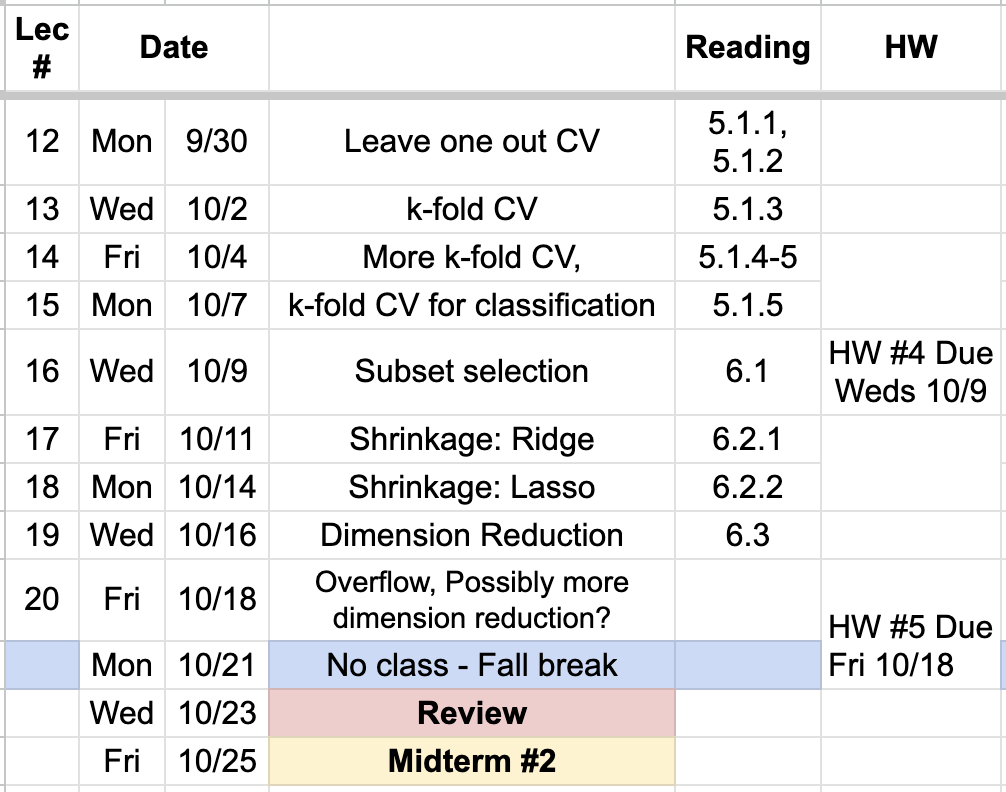
\includegraphics[align = c, width = .6\textwidth]{Day01-Schedule-Test2}


\end{frame}
%--- Next Frame ---%


\end{document}
